\chapter{Introdução}

% \MexerDepois{Escrever algo aqui}

Este capítulo conta com a motivação para o trabalho proposto, os objetivos gerais e secundários, e uma apresentação da estrutura geral do trabalho.

\section{Motivação}

O surgimento de problemas crônicos de saúde decorrentes à idade avançada vêm se tornando cada vez mais comum, já que a longevidade da população vem subindo \cite{medico24hs2021}.
Neste contexto, o número de pacientes que dependem de medicamentos de uso contínuo é cada vez mais alto, mas simultaneamente, estes podem ter problemas para identificar seus remédios \cite{porto2023}.
Com a idade avançada, também surgem problemas relacionados à visão, e surge a necessidade de alguma assistência para garantir que os medicamentos não sejam confundidos, o que poderia levar a danos na saúde do paciente \cite{ione2017}.

\subsection{Medicamentos de uso contínuo}

Cerca de \SI{52}{\percent} da população brasileira sofre de alguma doença crônica, como colesterol alto, diabetes ou hipertensão.
Apesar de muitas vezes não terem cura, são doenças tratáveis, geralmente com medicamentos de uso contínuo, que devem ser ministrados periodicamente, e sem previsão de interrupção no tratamento \cite{porto2023}.

Usualmente, são remédios de uso controlado, que exigem receita na hora da compra, dessa forma, também é necessário que os pacientes mantenham o acompanhamento médico em dia.
O \ac{SUS} oferece alguns programas para facilitar o acesso a alguns desses medicamentos, fornecendo gratuitamente ou num preço acessível \cite{porto2023}.

Mais de \SI{70}{\percent} desses pacientes não seguem corretamente a prescrição, em alguns casos até tendo efeitos diferentes dos esperados para tais medicamentos \cite{porto2023}.

\subsection{Embalagens de medicamentos}

Confundir medicamentos pode trazer sérios riscos à saúde, atualmente, é comum que laboratório utilizem elementos visualmente semelhantes nas embalagens, isso pode levar um paciente ao engano.
Tipografias semelhantes ou pequenas, problemas de contraste ou até nomes que possam induzir ao erro são alguns dos problemas presentes.
Em alguns casos, o farmacêutico precisa alertar o paciente que está levando o medicamento errado, em alguns outros, o paciente nota o erro um tempo depois e retornam à farmácia com objetivo de realizar a troca do produto \cite{ione2017}.

Há uma norma da \ac{Anvisa} que regulamenta a rotulagem de medicamentos, garantindo que novos registros não possam utilizar elementos visuais semelhantes ao de medicamentos registrados anteriormente.
Todavia, em alguns casos, o laboratório pode alterar o rótulo sem prévia aprovação da \ac{Anvisa} \cite{ione2017}.

Outro problema associado é automedicação, quando o paciente deliberadamente toma remédios sem uma prescrição médica.
Mais da metade da população brasileira tem o hábito de se automedicar.
Não somente casos onde o paciente deliberadamente utiliza o remédio sem prescrição, mas também casos onde, com a prescrição, alteram o período ou a posologia indicada pelo profissional da saúde \cite{crfsp2019}.

A automedicação pode disfarçar sintomas de doenças mais graves, isso atrapalha o profissional da saúde, atrasando o diagnóstico e tratamento apropriado.
O hábito de manter uma maleta com remédios em casa também tem grande influência, especialmente quando são utilizados remédios fora do prazo de validade ou quando se confunde um medicamento com outro pela semelhança da embalagem \cite{g12019}.


% https://www.crfsp.org.br/noticias/10535-pesquisa-aponta-que-77-dos-brasileiros-têm-o-hábito-de-se-automedicar.html


% http://www.cff.org.br/noticia.php?id=5279&titulo=Veja+a+repercuss%C3%A3o+da+pesquisa+sobre+uso+racional+de+medicamentos+na+m%C3%ADdia

% https://oglobo.globo.com/economia/defesa-do-consumidor/parece-mas-nao-o-perigo-de-remedios-com-caixas-similares-22059860
% https://www.pfizer.com.br/noticias/ultimas-noticias/os-riscos-da-automedicacao
% https://bvsms.saude.gov.br/bvs/premio_medica/pdfs/trabalhos/mencoes/januaria_ramos_trabalho_completo.pdf
% https://www.gov.br/Anvisa/pt-br/centraisdeconteudo/publicacoes/educacao-e-pesquisa/comunicacao-em-saude/campanha-a-informacao-e-o-melhor-remedio-cartilha.pdf
% https://site.cff.org.br/noticia/Noticias-gerais/23/04/2024/pesquisa-revela-que-9-entre-10-brasileiros-se-automedicam
% https://www1.folha.uol.com.br/equilibrioesaude/2019/04/quase-80-dos-brasileiros-se-automedicam-diz-pesquisa-datafolha.shtml

% \MexerDepois{Completar isso}

\subsection{Problemas de Visão em Idade Avançada}

A \ac{OMS} define como baixa visão o intervalo com acuidade visual abaixo de 20/60 (ou 6/18) e acima de 20/400 (ou 3/60) no melhor olho, após correção refrativa ou tratamento \cite{CBO2013condicoes}.
Este valor é referente ao teste ocular realizado utilizando um diagrama de Snellen a uma distância de 20 pés (\SI{6.1}{\metre}), a \autoref{fig:snellen_chart} ilustra o diagrama utilizado.
A visão é considerada com deficiência leve ou sem deficiência (20/20 ou 6/6) no caso que o paciente seja capaz de identificar os símbolos das linhas inferiores no diagrama \cite{lenscope2021}.

\begin{figure}[!htpb]
    \centering
    \caption{Diagrama de Snellen, fora de escala.}
    \label{fig:snellen_chart}
    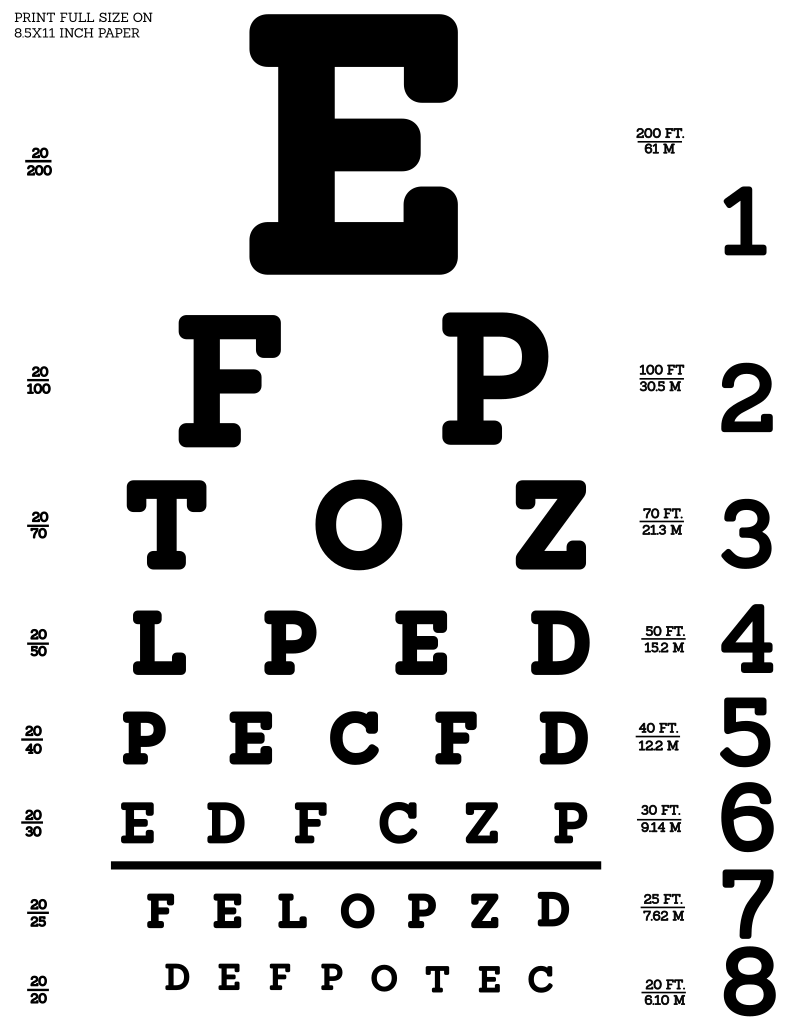
\includegraphics[keepaspectratio, width=\linewidth, height=0.75\textheight]{../pictures/Snellen_chart.png}
    \caption*{Fonte: \href{https://commons.wikimedia.org/wiki/File:Snellen_chart_by_Openclipart.svg}{Openclipart, CC0, via Wikimedia Commons}}
\end{figure}

A porcentagem de deficiência visual é distribuída de forma desigual entre faixas etárias.
Para crianças e adolescentes, na faixa de 5 a 15 anos, cerca de \SI{8}{\percent} apresentam alguma deficiência visual.
A proporção é de \SI{19}{\percent} para adultos em idade ativa, de 16 a 49 anos, enquanto para adultos com mais de 50 anos, \SI{75}{\percent} da população apresenta algum tipo de deficiência visual \cite{CBO2013condicoes}.

O aumento da expectativa de vida traz também o aumento no número de pessoas com baixa visão, já que a maior parte das doenças que podem causar alguma deficiência visual é desencadeada em idade avançada.
Presbiopia é o nome dado à perda da flexibilidade da acomodação do cristalino no olho, tal condição dificulta a capacidade de focalização de objetos em certas distâncias, e é a causa mais comum de deficiência visual em todo mundo.
Essa condição é classificada como erro refrativo, como miopia, hipermetropia e astigmatismo, e pode ser corrigida com óculo de leitura.
Em 2015, a Agência Internacional para a Prevenção da Cegueira estimou que cerca de \num{1,1} bilhão de pessoas, com 35 anos ou mais, tinham a visão afetada pela presbiopia, precisando usar óculos para perto.
Dessas, \num{677} milhões teriam 50 anos ou mais \cite{CBO2013condicoes}.


% \cite{CBO2013condicoes, lenscope2021}

\subsection{Tecnologia Assistiva}

No dia a dia, é comum a utilização de diversos tipos de tecnologias que tem como objetivo facilitar a vida dos usuários.
Atualmente, é difícil pensar na rotina sem alguns destes equipamentos, pois já fazem parte do cotidiano da vida moderna.
Desde tecnologias simples, como uma tesoura ou um óculos, a tecnologias mais complexas, como uma assistente virtual capaz de falar sobre o clima e as notícias do dia.
Destacam-se aqui tecnologias como cadeiras de rodas ou aparelhos auditivos, criadas especialmente com o objetivo de auxiliar pessoas que nasceram ou desenvolveram características que tornariam sua vida mais complicada.

É definido como \ac{TA} todo aparato que tem como objetivo prover habilidades funcionais para pessoa idosa ou com deficiência \cite{bersch2008introduccao}.
Essa definição abrange produtos, serviços, práticas, estratégias e instrumentos utilizados com o objetivo de prevenir, aliviar, compensar ou neutralizar as desvantagens, incapacidades ou deficiências dessas pessoas, provendo maior autonomia e qualidade de vida.

O uso de \acp{TA} simples pode ser tão antigo quanto a humanidade em si, pode se imaginar uma pessoa idosa andando com o apoio de um galho como uma bangala, ou como uma muleta para alguém machucado.
Existem casos de tecnologias que, originalmente, não tinha o objetivo de serem assistivas, como a ``Escrita Noturna'', que foi criada com o objetivo de trocar mensagens entre soldados que pudessem ser lidas a noite, mas foi posteriormente adotada para o Braille, e até hoje é usado como técnica de escrita para pessoas com deficiência visual \cite{sebold2020tecnologia}.
Mas também existem casos de tecnologias desenvolvidas com o objetivo de serem assistivas mas são utilizadas para ``facilitar'' a vida de quem não precisaria delas originalmente, como carros de câmbio automático.

Em novembro de 2006, foi criado no Brasil o Comitê de Ajudas Técnicas, que tem entre seus objetivos, propor e monitorar o cumprimentos de medidas associadas às \acp{TA} em seu âmbito prático
\cite{galvao2009tecnologia}.

% https://edisciplinas.usp.br/pluginfile.php/4097104/mod_resource/content/1/Aula%20mobilidade%20e%20transporte.pdf#:~:text=o%20Muletas%20e%20andadores%20são,ajudar%20as%20pessoas%20a%20caminhar.

% \cite{bersch2008introduccao, sebold2020tecnologia, galvao2009tecnologia}

\section{Objetivos}

O principal objetivo desde projeto é idealizar e desenvolver um sistema capaz de identificar o nome de um medicamento em uma embalagem e retornar ao usuário a bula digital correspondente.

Como objetivo secundário, desenvolver sistema capaz de lidar com imagens capturadas em diferentes contextos, que possa realizar leitura do texto nela inserido. Também buscar em um banco de bulas eletrônicas os termos encontrados na imagem.

% \MexerDepois{Completar isso depois}

\section{Estrutura do documento}

% \MexerDepois{Completar isso depois}

O trabalho proposto está organizado em cinco capítulos, apresentando, após este introdutório, mais quatro capítulos. O \autoref{cap:revbib} traz um levantamento bibliográfico, contendo fundamentação teórica e revisão de trabalhos relacionados. O \autoref{cap:metodologia} apresenta o detalhe da metodologia adotada na construção do trabalho. No \autoref{cap:resultados} são apresentados detalhes sobre banco de imagens construído, detalhes sobre a performance e problemas encontrados. Por fim, o \autoref{cap:conclusao} traz as considerações finais, conclusões e levantamentos para trabalhos futuros que podem resultar em melhorias na presente proposta.

O documento também conta com o \autoref{apdx:codigo}, que apresenta o condjunto de códigos utilizados ao longo do desenvolvimento do trabalho.
